\chapter{Stato dell'arte}
\label{statodellarte}
In questo capitolo saranno mostrati i fondamenti teorici su cui è basato il lavoro presentato all'interno di questo elaborato.... ><<<<><<<

\newpage
\section{Machine Learning}
\label{machinelearning}
Il Machine Learning è un sottocampo dell'intelligenza artificiale (IA) è stato definito da Arthur Samuel nel 1959 \cite{5392560}. L'obiettivo del machine learning generalmente è capire la struttura dei dati e adattare tali dati in modelli in grado di essere capiti e utilizzati da utenti.

Nonostante il Machine Learning sia un campo informatico, si differenzia dai tradizionali approcci computazionali. Nell'informatica tradizionale, gli algoritmi sono serie di istruzioni programmate esplicitamente usate dai calcolatori per elaborare dati o risolvere problemi. Gli algoritmi Machine Learning, al contrario, permettono ai calcolatori di allenarsi su input di dati ed usare analisi statistica in modo da produrre valori che ricadono all'interno di intorni specifici. Grazie a questo, il machine learning facilita ai calcolatori la costruzione di modelli che siano in grado di automatizzare processi decisionali basati su campioni di dati.

Molti campi tecnologici odierni sfruttano i benefici del machine learning; ad esempio tecnologie di riconoscimento facciale permettono alle piattaforme di social networks di aiutare gli utenti nel tag delle foto di amici. Altro esempio sono le tecnologie di Optical Character Recognition (OCR) in grado di convertire immagini di testi stampati in documenti testuali modificabili da un word processor. I recommendation engines, basati su machine learning, suggeriscono agli utenti i programmi televisivi o film basati sulle loro preferenze. Le auto a guida autonoma si basano su machine learning in molte applicazioni, ad esempio per il riconoscimento della segnaletica stradale.

Nel machine learning i compiti sono generalmente classificati in grandi categorie. Tali categorie sono basate su come l'apprendimento è impostato o su come il feedback dell'apprendimento viene dato al sistema.

Due dei metodi di apprendimento più comunemente adottati sono l'apprendimento supervisionato in cui si allenano algoritmi basandosi su input e output di esempio, categorizzati da esseri umani e l'apprendimento non supervisionato, in cui non vengono forniti dati categorizzati agli algoritmi in modo da permettere al sistema di trovare autonomamente la struttura che compone i dati di input. Nelle sezioni seguenti si mostrano tali metodi in dettaglio.

\subsection{Tipologie di Problemi}
Il machine learning è impiegato principalmente per la risoluzione di tre tipologie di problemi:
\begin{itemize}
\item \textbf{classificazione}, quando è necessario decidere a quale categoria appartiene un determinato dato. Ad esempio per l'identificazione di specie di piante fornendo un'immagine.
\item \textbf{raggruppamento} (clustering), quando si vuole raggruppare i dati che presentano caratteristiche simili. Ad esempio, un sistema può raggruppare immagini di figure geometriche separando figure con 4 lati e i cui angoli sono a 90 gradi oppure tutte le figure con quattro lati in cui solo due sono paralleli, ecc. In marketing, ad esempio, il raggruppamento viene utilizzato per l'individuazione di clienti e mercati potenziali.
\item \textbf{regressione}, cioè prevedere il valore futuro di un dato avendo noto il suo valore attuale. Un esempio è la previsione della quotazione delle valute o delle azioni di una società. Nel marketing viene utilizzato per prevedere il tasso di risposta di una campagna sulla base di un dato profilo di clienti; nell’ambito commerciale per stimare come varia il fatturato dell’azienda al mutare della strategia.
\end{itemize}

\subsection{Apprendimento Supervisionato}
Nell'apprendimento supervisionato, vengono forniti al sistema dei dati di input già etichettati con l'output desiderato. Lo scopo di tale metodo è permettere all'algoritmo di apprendimento di imparare comparando il suo output con quello fornito in ingresso, in modo da rilevare errori e modificare il modello di conseguenza. L'apprendimento supervisionato perciò usa patterns per predire i valori delle "etichette" su dati non etichettati.

Ad esempio, con l'apprendimento supervisionato, si può fornire ad un algoritmo un insieme di immagini di squali, etichettati come $pesce$ e immagini di oceani etichettati come $acqua$. Allenandosi su tali dati, l'algoritmo supervisionato dovrebbe essere in grado di riconoscere immagini di squali ed etichettarle come $pesci"$ ed immagini di oceani ed etichettarle come $acqua$.

Un comune uso dell'apprendimento supervisionato è l'uso di dati storici per predire probabili eventi futuri. Può usare informazioni statistiche sull'andamento del mercato azionario ed anticipare fluttuazioni future o utilizzato per filtrare email di spam. E' possibile utilizzare foto di cani etichettate per identificare la razza di un cane unicamente dalla sua foto.

\subsection{Apprendimento non Supervisionato}
Nell'apprendimento non supervisionato, i dati non sono etichettati. L'algoritmo viene lasciato libero di rilevare affinità tra i dati di input. Siccome i dati non classificati sono molto piu comuni che grandi quantità di dati etichettati, i metodi di machine learning che facilitano l'apprendimento non supervisionato sono considerabili come molto pregiati.

L'obiettivo dell'apprendimento non supervisionato può essere diretto, come la ricerca di pattern nascosti all'interno dei dati, ma può anche avere l'obiettivo di \textit{feature learning}: l'apprendimento di caratteristiche particolari che permette al sistema di scoprire automaticamente le rappresentazioni necessarie a classificare i dati grezzi.

L'apprendimento non supervisionato viene comunemente utilizzato per dati transazionali. Ad esempio, nel caso reale di un grosso dataset di clienti e dei loro acquisti, un essere umano difficilmente riuscirebbe a ricavare gli attributi che legano i profili clienti e le tipologie dei loro acquisti. Tuttavia fornendo tali dati ad un algoritmo di  apprendimento non supervisionato è possibile rilevare caratteristiche che legano determinati gruppi di clientela a determinati prodotti e di conseguenza prendere decisioni di marketing mirate.

L'apprendimento non supervisionato, grazie alla mancanza di un target da raggiungere, è in grado di analizzare dati che   apparentemente non mostrano relazioni ed estrarne dati significativi. Viene spesso usato per eseguire \textit{anomaly detection}, come l'utilizzo fraudolento di carte di credito; oppure è possibile eseguire classificazione di immagini (come nel precedente caso di razze canine) in maniera autonoma partendo da immagini non categorizzate.

\subsection{Apprendimento Semi Supervisionato}
Posto a metà tra il supervisonato e il non-supervisionato, l’apprendimento parzialmente supervisionato si basa su dati misti in cui una minima parte è già etichettata e una larghissima maggioranza è costituita da dati non etichettati.  Questo approccio viene utilizzato per migliorare le previsioni fatte dalla macchina sui dati non etichettati e richiede, normalmente, l’intervento di un analista. L’approccio è principalmente usato nei problemi di classificazione e di raggruppamento o nella descrizione delle relazioni causa-effetto tra le variabili.

\subsection{Apprendimento per Rinforzo}
L'apprendimento per rinforzo (Reinforcement learning) è una tecnica di apprendimento automatico che punta a realizzare sistemi in grado di apprendere ed adattarsi ai cambiamenti dell’ambiente in cui sono immersi attraverso la distribuzione di una “ricompensa” detta rinforzo, data dalla valutazione delle prestazioni.
Il suo funzionamento è attuato da tre componenti:
\begin{itemize}
\item un sistema logico di esecuzione (definito A), che sulla base dei dati in ingresso (Input) riesce a restituire un risultato (Output)
\item un sistema logico di valutazione (definito B) che assegna un premio (se il risultato è corretto) o una penalità (se il risultato non è corretto) al sistema logico A
\item un sistema logico di ottimizzazione (definito C) che osserva il comportamento di A e B e modifica il modello utilizzato da A per aumentare il premio e ridurre le penalità che B assegna ad A.
\end{itemize}

L’apprendimento per rinforzo è utilizzato in tutti quei campi in cui è essenziale che la macchina risponda ai cambiamenti dell’ambiente. Per questo è utilizzato frequentemente nella robotica, per controllare i movimenti degli automi, ma anche nelle auto a guida autonoma. Trova anche applicazione in ambiti industriali nella produzione e nel controllo qualità e in diversi altri settori.



\newpage
\section{Deep Learning e Reti neurali}
Il Deep Learning è uno specifico sottocampo del machine learning, un diverso modo di apprendere rappresentazioni di dati, principalmente orientato verso l'apprendimento di successivi strati (\textit{layers}) di rappresentazione via via più significativi. Il termine "deep" indica la presenza di questa moltitudine di strati che compongono il modello
di rappresentazione dei dati; infatti il deep learning odierno comprende generalmente modelli composti da decine o centinaia di strati successivi di rappresentazione, i quali apprendono in maniera automatica tramite l'esposizione ai dati di allenamento. Per confronto, gli approcci di machine learning descritti in sezione \ref{machinelearning} generalmente coinvolgono uno o due strati di rappresentazione dei dati. Difatti tali modelli vengono definiti anche come \textit{shallow learning}.
 
\begin{figure}[htbp]
	\centering
	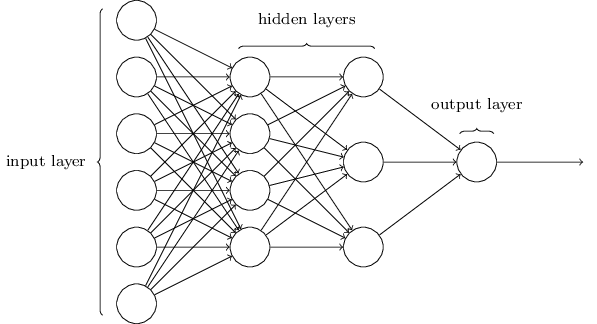
\includegraphics[width=\columnwidth]{figures/mlp-network.png}
	\caption{Schema generico di una rete Neurale \label{nn}}
\end{figure} 
 
All'interno del deep learning, queste rappresentazioni a più strati sono quasi unicamente apprese attraverso modelli definiti \textbf{reti neurali}, strutturati letteralmente in strati sovrapposti gli uni agli altri. Il termine "rete neurale" deriva dal campo della neurobiologia, tuttavia non si tratta di veri e propri modelli del funzionamento del cervello umano.

\begin{figure}[!bp]
	\centering
	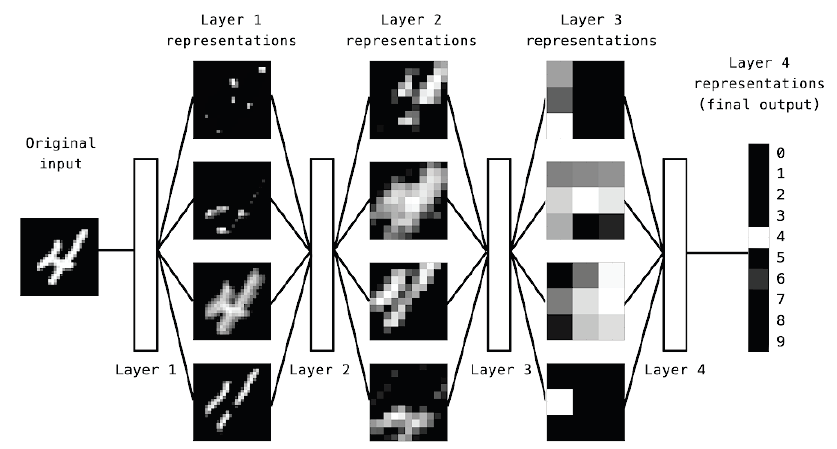
\includegraphics[width=\columnwidth]{figures/deeplearning.png}
	\caption{Esempio di rappresentazione di una cifra numerica tramite rete neurale. \textit{fonte}%
	 \cite{chollet2017deep} \label{fig:neuralnetwork} }
\end{figure}

Come è possibile vedere in figura \ref{fig:neuralnetwork}, la rete neurale trasforma l'immagine di una cifra numerica disegnata a mano in una rappresentazione via via più informativa riguardo il risultato finale. Si può considerare il deep leraning come una operazione di distillazione di informazioni composta da più fasi in cui i dati vengono filtrati in maniera sempre più fine.

\subsection{Funzionamento Reti Neurali}
Le informazioni specifiche riguardo quali operazioni un livello apporta ai dati di input sono immagazzinate all'interno degli strati stessi, nella matrice dei "pesi". La trasformazione implementata da un livello è parametrizzata da tali pesi. Generalmente la fase di apprendimento consiste nel trovare un set di valori per i quali i pesi di tutti gli strati che compongono una rete neurale mappino correttamente i dati di esempio ai loro target associati.
Tuttavia l'operazione di ricerca dei valori ottimali non è triviale, in quanto una rete neurale può contenere fino a decine di milioni di parametri e rilevarne i valori corretti risulta in una operazione complessa.

Per superare tale vincolo, la fase di apprendimento di una rete neurale è composta da più fasi di osservazione, nel quale si misura quanto distante si trova l'output da quanto atteso. Tale è il compito della funzione di \textit{loss}. La funzione di loss utilizza la predizione della rete neurale e l'output atteso e computa un punteggio di distanza, catturando quindi la performance della rete sull'esempio analizzato.

Il meccanismo principale nel deep learning è l'uso di questo punteggio come segnale di \textit{feedback} per aggiustare il valore dei pesi in maniera da diminuire il valore del punteggio di loss per l'esempio analizzato. Questo aggiustamento è compito dell'\textit{ottimizzatore}, il quale implementa l'algoritmo di \textit{backpropagation} che attua la modifica dei pesi durante la fase di apprendimento.

Inizialmente i pesi della rete neurale sono assegnati a valori randomici, causando per le prime fasi di apprendimento un valore di loss particolarmente alto. Via via che le fasi di apprendimento mostrano diversi esempi alla rete i pesi vengono aggiustati di una piccola parte nella direzione corretta, causando una decrescita nel punteggo di loss. Questo \textit{training loop} viene ripetuto per un numero sufficiente di volte fino al raggiungimento di un valore minimo di loss e alla produzione di output il più possibile simile a quello desiderato. In figura \ref{fig:neuralloss} è mostrato uno schema di alto livello.

\begin{figure}[!htbp]
	\centering
	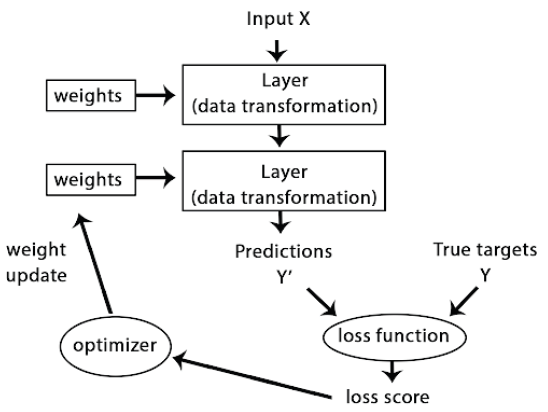
\includegraphics[width=0.8\columnwidth]{figures/deeploss.png}
	\caption{Schema di alto livello del funzionamento di una rete neurale. \textit{fonte}%
	 \cite{chollet2017deep} \label{fig:neuralloss} }
\end{figure}


\newpage
\section{Adversarial Learning}
Le tecniche di machine learning possono essere utilizzate per prevenire azioni vietate o illegali e nel caso vi siano degli incentivi economici, vi possono essere probabili antagonisti intenzionati ad eludere tali restrizioni. Un esempio tipico è il caso del filtraggio anti spam, nel quale gli spammers forgiano messaggi ad hoc per eludere le più recenti tecniche di filtraggio. Tali tecniche possono essere identificate come \textit{adversarial learning} (apprendimento antagonista).

Le vulnerabilità dei metodi di machine learning rispetto a manipolazione antagonista non possono venire semplicemente ignorate con la richiesta di tecniche più "robuste". I fondamenti teorici del machine learning odierno sono largamente costruiti sull'assunto che i dati di allenamento descrivano adeguatamente la realtà del fenomeno studiato. Questo assunto viene chiaramente violato nel caso che le distribuzioni di allenamento o di test vengano alterate, assumendo che gli antagonisti utilizzino qualsiasi mezzo possibile per disturbare l'algoritmo di apprendimento. I metodi di apprendimento in caso di ambienti antagonisti dovrebbero quindi essere in grado di sostenere una distorsione nei propri dati.

Come dimostrato da ricerche precedenti ( \cite{kearnsli}, \cite{Auer2002}, \cite{paclearning} ) un antagonista senza vincoli che può arbitrariamente alterare dati e target, può introdurre un errore fino al 100\%. Tuttavia nei casi pratici gli attackers devono atteneresi a determinati vincoli; ad esempio una email di spam deve recapitare il suo messaggio, un malware inviato ad un host deve eseguire correttamente e sfruttare una vulnerabilità e antagonisti che cercano di alterare i motori di ricerca possono controllare solo una frazione di tutti i domini raggiungibili. In alcuni casi si può mostrare come certi vincoli possono rendere la rilevazione di un attacco computazionalmente intrattabile \cite{fogla}.

L'investigazione di metodi di machine learning per ambienti ostili è stata attuata in tre aree di ricerca largamente distinte: machine learning, sicurezza informatica e spam filtering. Nel caso di machine learning ricerche precedenti si sono incentrate su metodi di minimo-massimo con l'obiettivo di ottenere robustezza rispetto alla incertezza dell'input. Ad esempio classificatori più robusti sono stati sviluppati per gestire casi come il feature deletion \cite{globerson} ; oppure ricerche hanno dimostrato che equilibri unici di Nash esistono per alcune tipologie di situazioni antagoniste \cite{nash} .

Una differente visione dei problemi di apprendimento antagonista è emersa nel campo della sicurezza informatica, specialmente per quel che riguarda il rilevamento di intrusioni (\textit{intrusion detection} ). Diversi metodi sono stati proposti per rilevare pacchetti di rete anomali o per generare automaticamente \textit{signatures} strettamente legate a metodi di machine learning (ad esempio i lavori eseguiti in \cite{wangstolfo} e \cite{wang2006} ).

L'area dello spam filtering ha richiesto sforzi fondamentali da parte degli esperti in sicurezza; la costante ricerca di tecniche di evasione dei filtri anti-spam ha portato a studi estensivi riguardo vincoli e tecniche robuste di filtering \cite{dalvi}. 

Il machine learning può fornire soluzione a difficili problemi di sicurezza di rete, compresi filtri anti-spam, rilevazione di vari tipologie di attacchi contro server e host, rilevazione di pagine web 
deliberatamente modificate per manipolare i motori di ricerca sfruttandone le vulnerabilità. Tutte queste problematiche riguardano la manipolazione di grandi quantità di dati in un ambiente altamente variabile e il bisogno di tecniche di classificazione veloci ed accurate. L'esistenza di antagonisti che possono trarre profitto in queste aree complica l'applicazione di machine learning e crea una "corsa agli armamenti" tra chi sviluppa classificatori sempre piu robusti e antagonisti che cercano di manipolare tali classificatori. Fortunatamente ogni area di applicazione fornisce vincoli riguardo le azioni antagoniste che rendono la classificazione fattibile. 

\begin{figure}[!htbp]
	\centering
	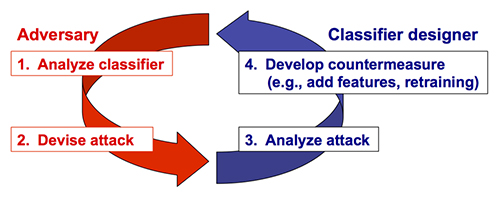
\includegraphics[width=\columnwidth]{figures/Reactive_arms_race.jpg}
	\caption{Schema concettuale del rapporto tra difensori ed antagonisti. \textit{fonte}%
	 \cite{wiki:Adversarial_machine_learning} \label{fig:advarms} }
\end{figure}


\subsection{Adversarial Networks}
The adversarial modeling framework is most straightforward to apply when the models are both multilayer perceptrons. To learn the generator's distribution $p_g$ over data $\bm{x}$, we
define a prior on input noise variables $p_{\bm{z}}(\bm{z})$, then represent a
mapping to data space as $G(\bm{z}; \theta_g)$, where $G$ is a differentiable function
represented by a multilayer perceptron with parameters $\theta_g$. We also define a second
multilayer perceptron $D(\bm{x}; \theta_d)$ that outputs a single scalar. $D(\bm{x})$ represents
the probability that $\bm{x}$ came from the data rather than $p_g$. We train $D$ to maximize the
probability of assigning the correct label to both training examples and samples from $G$.
We simultaneously train $G$ to minimize $\log(1-D(G(\bm{z})))$:

In other words, $D$ and $G$ play the following two-player minimax game with value function $V(G, D)$: 

\begin{equation}
\label{eq:minimaxgame-definition}
\min_G \max_D V(D, G) = \mathbb{E}_{\bm{x} \sim p_{\text{data}}(\bm{x})}[\log D(\bm{x})] + \mathbb{E}_{\bm{z} \sim p_{\bm{z}}(\bm{z})}[\log (1 - D(G(\bm{z})))].
\end{equation}

In the next section, we present a theoretical analysis of adversarial nets,
essentially showing that the training criterion allows one to recover the data
generating distribution as $G$ and $D$ are given enough capacity, i.e., in the
non-parametric limit. See Figure~\ref{fig:intuition} for a less formal, more pedagogical
explanation of the approach.
In practice, we must implement the game using an iterative, numerical approach. Optimizing $D$ to completion in the
inner loop of training is computationally prohibitive,
and on finite datasets would result in overfitting. Instead, we alternate between $k$ steps
of optimizing $D$ and one step of optimizing $G$. This results in $D$ being maintained
near its optimal solution, so long as $G$ changes slowly enough. This strategy is analogous
to the way that SML/PCD~\citep{Younes1999,Tieleman08} training maintains samples from a Markov chain from one
learning step to the next in order to avoid burning in a Markov chain as part of the inner loop
of learning. The procedure is formally presented
in Algorithm~\ref{alg:AGF}.

In practice, equation~\ref{eq:minimaxgame-definition} may not provide sufficient gradient for $G$ to learn
well. Early in learning, when $G$ is poor, $D$ can reject samples with high confidence because they are
clearly different from the training data. In this case, $\log ( 1- D(G(\bm{z})))$ saturates. Rather than
training $G$ to minimize $\log (1 - D(G(\bm{z})))$ we can train $G$ to maximize $\log D(G(\bm{z}))$.
This objective function results in the same fixed point of the dynamics of $G$ and $D$ but provides much
stronger gradients early in learning.


%explains the intuition
%behind these asymptotic consistency results. When $D$ tracks its optimum,
%it classifies $x$'s according to Bayes rule, i.e., 
%$D^*(x) = \frac{P_X}{P_X(x) + P_G(x)}$, and the gradient of $D(G(z))$ on $G(z)$ pushes
%probability mass in the direction of increasing value of $D$, i.e., towards regions 
%where $P_X(x)>P_G(x)$. This necessarily pulls probability mass away from
%regions where $P_X(x)<P_G(x)$. This happens because on the border of regions
%where $P_X(x)>P_G(x)$ the derivative of $D^*$ must point inside, and vice-versa.
%Hence the gradient pushes $G$ towards allocating more mass where it did not put enough,
%and vice-versa. A more formal proof of convergence is presented in Section~\ref{},
%also showing that the criterion is consistent, so long as $D$ is allowed to track
%its optimum, i.e., $G$ is making small changes between optimizations of $D$.

\begin{figure}[h]
\begin{tabular}{m{3cm}m{3cm}m{3cm}m{0.1cm}m{3cm}}
    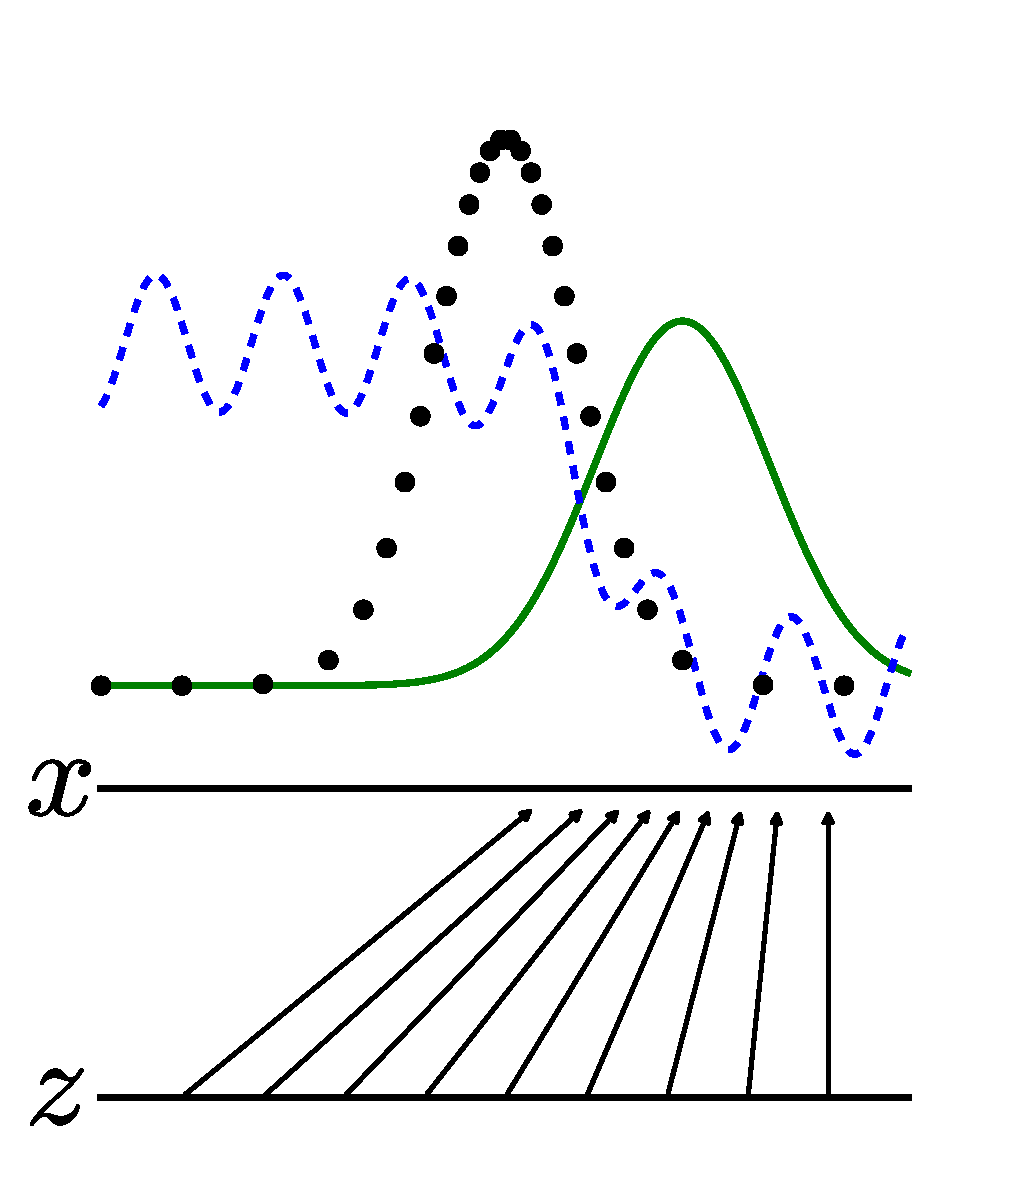
\includegraphics[width=3cm, height=4cm]{fig1.pdf} 
    &  
    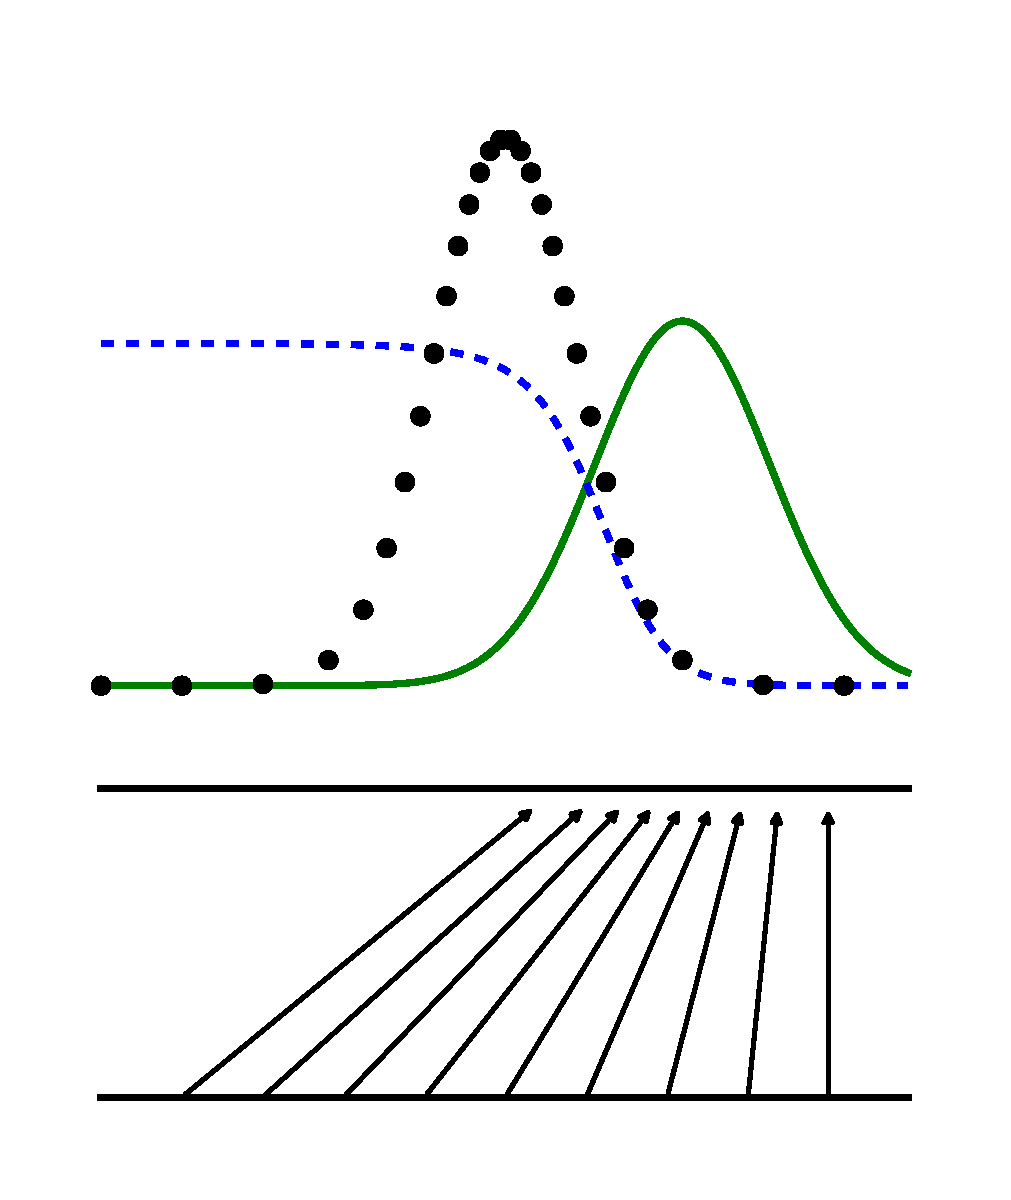
\includegraphics[width=3cm, height=4cm]{fig2.pdf}
    & 
    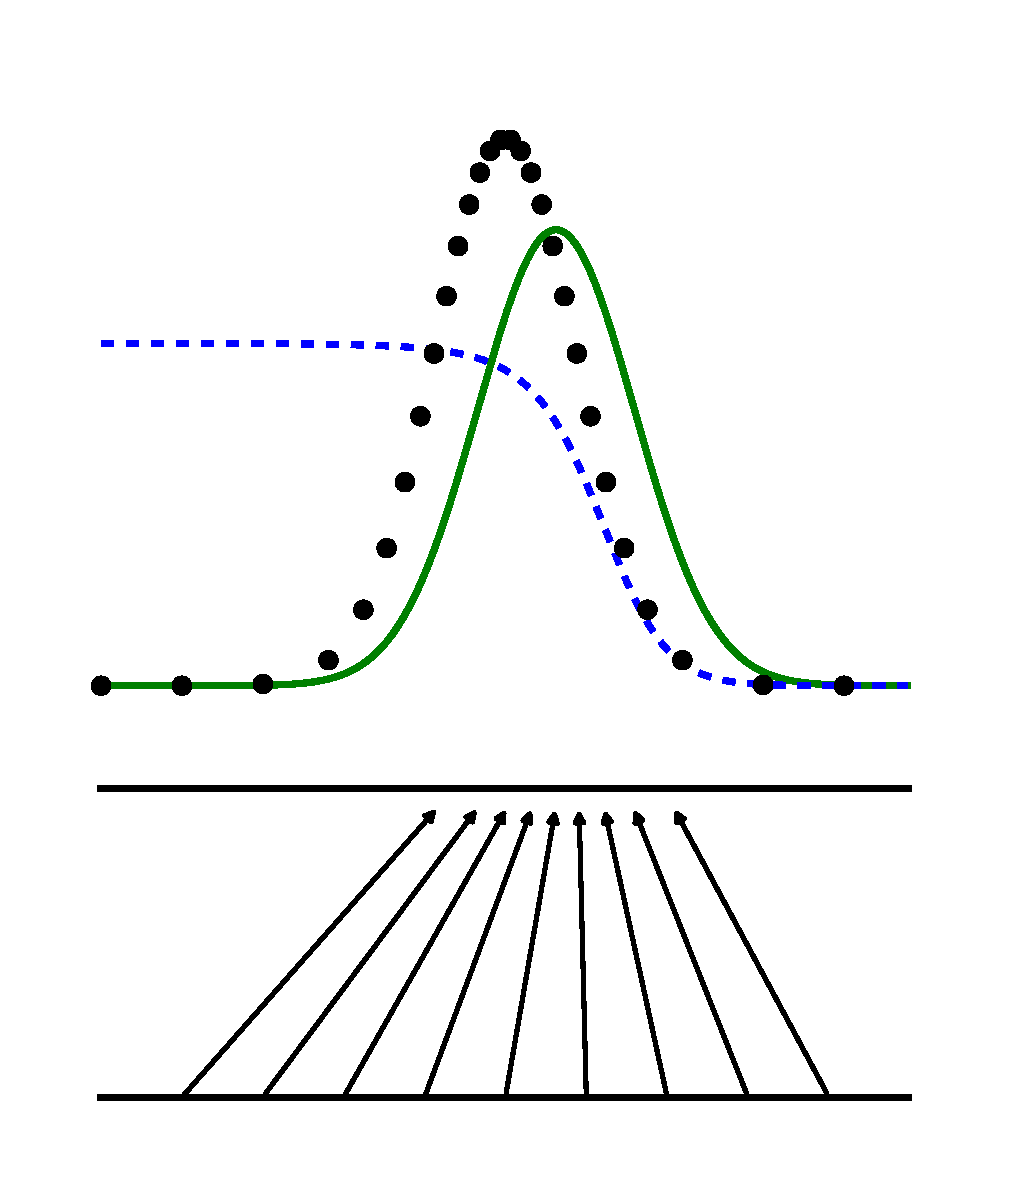
\includegraphics[width=3cm, height=4cm]{fig3.pdf}
    &
    \dots
    &
    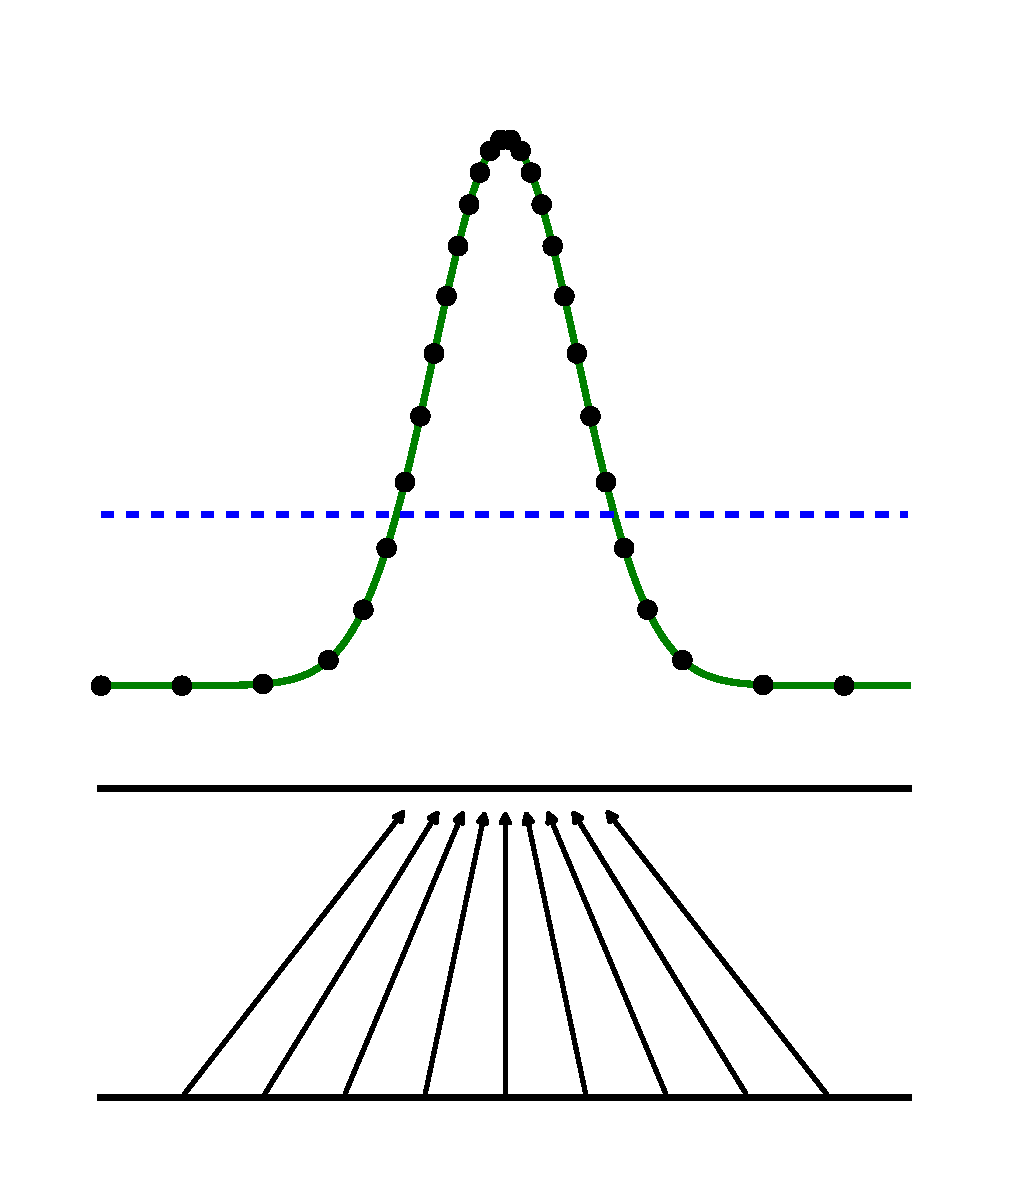
\includegraphics[width=3cm, height=4cm]{fig4.pdf}
    \\
    \centering (a)
    & 
    \centering (b) 
    & 
    \centering (c) 
    &  
    & 
    \centering (d)
\end{tabular}

\caption{\small
Generative adversarial nets are trained by simultaneously updating the \textbf{d}iscriminative 
distribution ($D$, blue, dashed line) so that it discriminates between samples from
the data generating distribution (black, dotted line)
$p_{\bm{x}}$ 
from those of the \textbf{g}enerative distribution $p_g$ (G) (green, solid line).
The lower horizontal line is the domain from which $\bm{z}$ is sampled, in this case uniformly.
The horizontal line above is part of the domain of $\bm{x}$. The upward arrows show
how the mapping $\bm{x}=G(\bm{z})$ imposes the non-uniform distribution $p_g$ on transformed samples.
$G$ contracts in regions of high density and expands in regions of low density of $p_g$.
(a) Consider an adversarial pair near convergence: $p_g$ is similar to $p_\text{data}$ and
$D$ is a partially accurate classifier.
(b) In the inner loop of the algorithm $D$ is trained to discriminate samples from data,
converging to
$D^*(\bm{x}) = 
\frac{
    p_\text{data}(\bm{x})
    }{
        p_\text{data}(\bm{x}) + p_g(\bm{x})}
$. 
(c) After an update to $G$, gradient of $D$ has guided $G(\bm{z})$ to flow to regions that are more likely
to be classified as data.
(d) After several steps of training, if $G$ and $D$ have enough capacity, they will reach a point at which
both cannot improve because $p_g = p_\text{data}$.
The discriminator is unable to differentiate between the two 
distributions, i.e. $D(\bm{x}) = \frac{1}{2}$.
}
\label{fig:intuition}
\end{figure}



\begin{algorithm}[ht]
\caption{\small Minibatch stochastic gradient descent training of generative adversarial nets.
The number of steps to apply to the discriminator, $k$, is a hyperparameter. We used $k=1$, the
least expensive option, in our experiments.
}
\begin{algorithmic}
\label{alg:AGF}
\FOR{number of training iterations}
  \FOR{$k$ steps}
    \STATE{$\bullet$ Sample minibatch of $m$ noise samples $\{ \bm{z}^{(1)}, \dots, \bm{z}^{(m)} \}$ from noise prior $p_g(\bm{z})$.}
    \STATE{$\bullet$ Sample minibatch of $m$ examples $\{ \bm{x}^{(1)}, \dots, \bm{x}^{(m)} \}$ from data generating distribution $p_\text{data}(\bm{x})$.}
    \STATE{$\bullet$ Update the discriminator by ascending its stochastic gradient:
        \[
            \nabla_{\theta_d} \frac{1}{m} \sum_{i=1}^m \left[
            \log D\left(\bm{x}^{(i)}\right)
            + \log \left(1-D\left(G\left(\bm{z}^{(i)}\right)\right)\right)
            \right].
        \]}
    %parameters $\theta_d$ of discriminator $D$
   %in the direction of the stochastic gradient of the binomial cross-entropy
   %for $D$ predicting whether its argument comes from $p_\text{data}(\bm{x})$ (target = 1, input = $\bm{x}$) or
   %$P_g$ (target = 0, input = $G(\bm{z})$), i.e., towards minimizing
   % \mbox{$-\log D(\bm{x}) - \log(1 - D(G(\bm{z})))$}.}
   \ENDFOR
  \STATE{$\bullet$ Sample minibatch of $m$ noise samples $\{ \bm{z}^{(1)}, \dots, \bm{z}^{(m)} \}$ from noise prior $p_g(\bm{z})$.}
    \STATE{$\bullet$ Update the generator by descending its stochastic gradient:
        \[
            \nabla_{\theta_g} \frac{1}{m} \sum_{i=1}^m
            \log \left(1-D\left(G\left(\bm{z}^{(i)}\right)\right)\right)
            .
        \]}
  \ENDFOR
  \\The gradient-based updates can use any standard gradient-based learning rule. We used momentum in our experiments.
\end{algorithmic}
\end{algorithm}

\subsubsection{Autoencoder}

